\documentclass[10pt]{unlsilabsop}
\title{IV test of bare modules}
\date{July 18, 2014}
\author{Frank Meier Aeschbacher}
\approved{Frank Meier Aeschbacher}
\sopid{203}
\sopversion{v0}
\sopabstract{Describes the procedure for the IV test of bare modules.}
\begin{document}

\maketitle

%------------------------------------------------------------------
\section{Scope}
This test is used for characterizing bare modules prior to assembly. In routine, this is part of the entry inspection after receiving new bare modules from the supplier.

This procedure shall not be used for fully assembled modules.

%------------------------------------------------------------------
\section{Purpose}
The IV curve is a critical parameter to check for the sanity of the sensor.

%------------------------------------------------------------------
%\section{Definitions}
%\begin{itemize}
%\item \textbf{bla} Text
%\end{itemize}

%------------------------------------------------------------------
%\section{Responsibilities}

%------------------------------------------------------------------
\section{Equipment}

\begin{itemize}
\item \textbf{Probe station} Jmicro JR-2745, to hold the setup
\item \textbf{Micropositioner} Jmicro KRN-09S, magnetically hold on the probe station, 2 pieces
\item \textbf{Pico probe model 7} mounted on microspositioner, used for GND connection
\item \textbf{Pico probe model 7A} mounted on micropositioner, used for HV connection
\item \textbf{Probe tips} Model 7-125, one for each pico probe
\item \textbf{Computer} Requires pXar installed
\item \textbf{DTB} Connected to the computer through a USB cable. No need to connect anything else, DTB just required for pXar to work properly.
\item \textbf{HV power supply} Keithly model 2430, connected to the same computer through a USB to RS232 adapter
\item \textbf{Connection box} to make proper connection between picoprobes and HV power supply
\item \textbf{Dark box} custom made dark PVC box
\item \textbf{Vacuum chuck} custom made, used to release modules off the GelPak
\item \textbf{Vacuum pen} connected to probe station, use it for manipulating bare modules
\end{itemize}

%------------------------------------------------------------------
\section{Setup}

Prepare the setup as shown in the image (TODO: add image)

%------------------------------------------------------------------
\section{Procedures}

\begin{enumerate}
\item Handle bare modules only with proper protection: ESD wristband, gloves, face mask.
\item Make sure the HV power supply is set to 0\,V.
\item Place the GelPak on the chuck, enable vacuum.
\item Use the vacuum pen to transfer the module to the probe station.
\item Make connections to the bare module according to the following image and table

\begin{tabular}{p{0.5\textwidth}p{0.5\textwidth}}
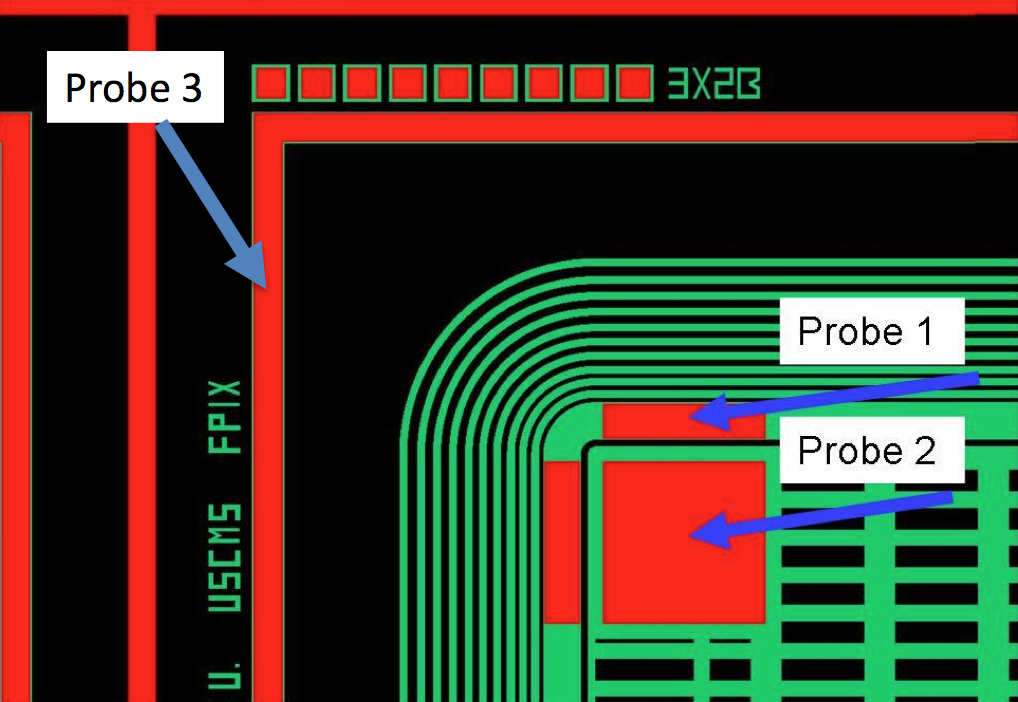
\includegraphics[width=0.5\textwidth]{img/SensorProbePositions.png} &
The image shows the areas on a sensor suitable for making an electrical contact in red.
\end{tabular}

\begin{tabular}{ll}
Area & Connect to \\
Probe 1 & Not used \\
Probe 2 & Connect to HV \\
Probe 3 & Connect to GND \\
\end{tabular}
\item By watching the probes under the microscope, make sure the probes touch the areas properly, especially the GND connection
\item Cover the setup using the dark box
\item Start the IV test in pXar
\item Upon finishing in pXar, save the image. Document the results according to the instructions below
\item Transfer module back to GelPak (if module goes back to storage) or place it on chuck (if module will be used immediately for assembly)
\end{enumerate}

%------------------------------------------------------------------
\section{Documentation}
The following information needs to be recorded:
\begin{itemize}
\item pXar: version number
\item HV power supply: serial number
\item test results from pXar
\end{itemize}


\end{document}

